\begin{figure}[H]
    \centering
    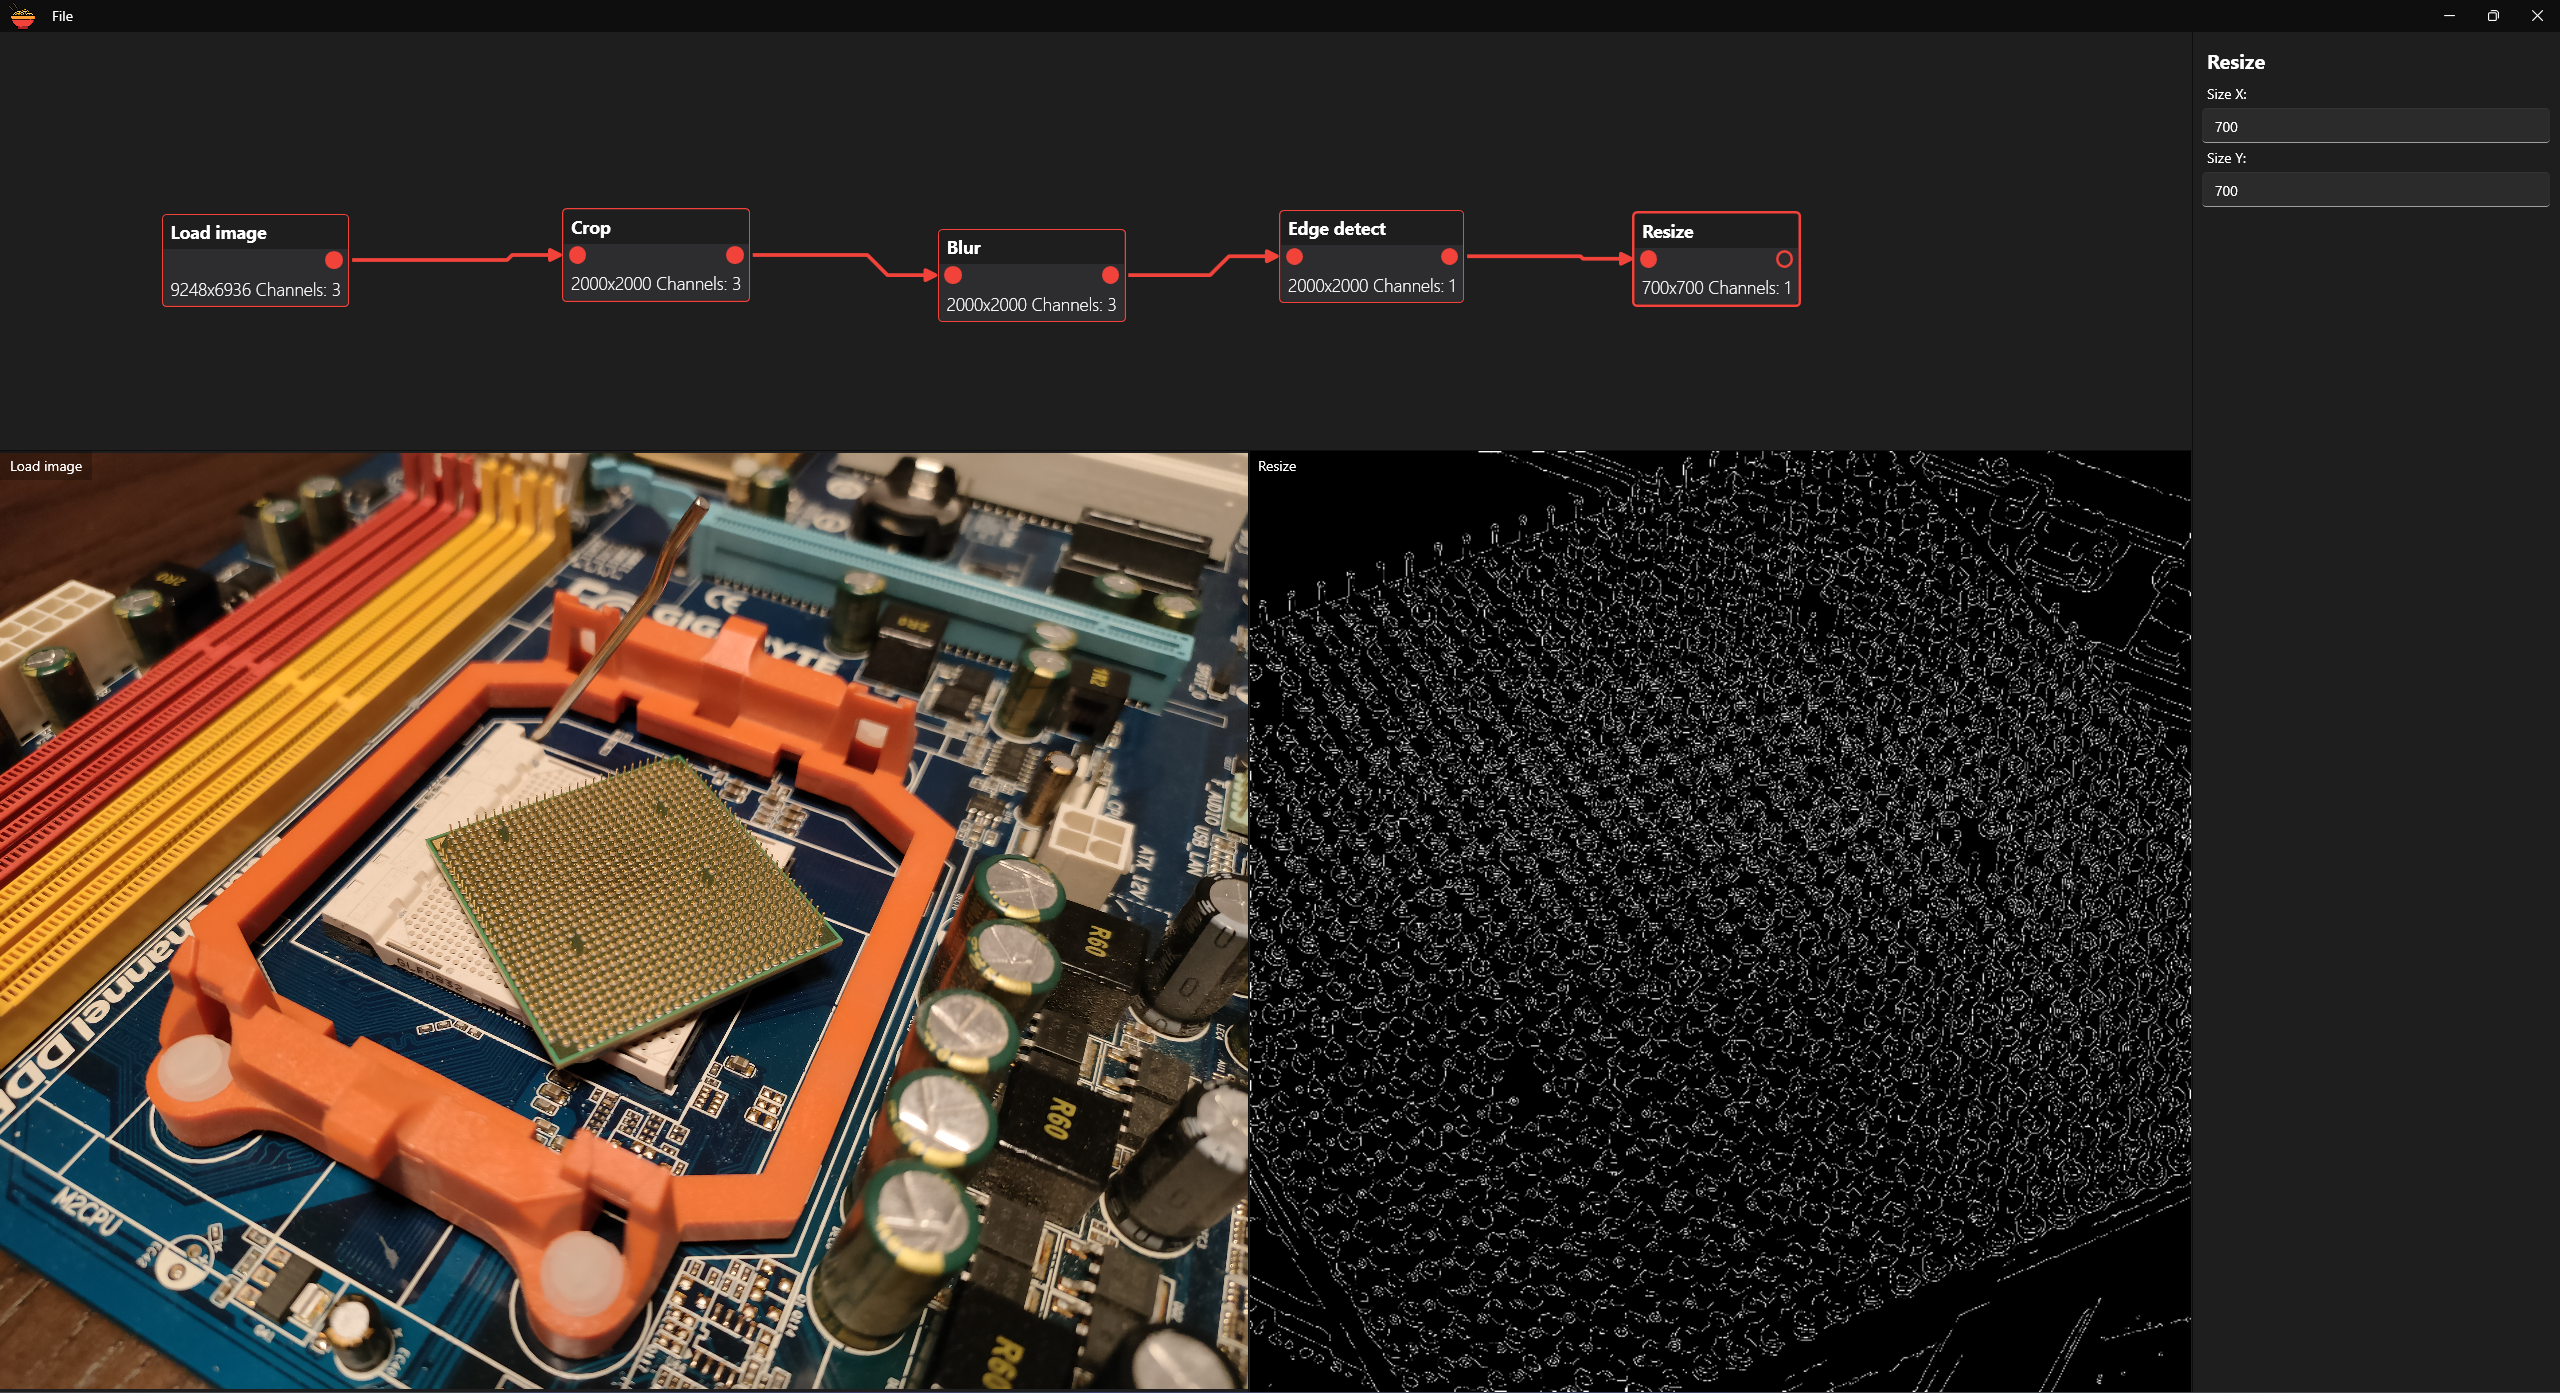
\includegraphics[width=1\linewidth]{images/Picture27.png}
    \caption{Wykrywanie krawędzi na wybranym fragmencie obrazu. Opracowanie własne.}
    \label{fig:socket}
\end{figure} 

\begin{figure}[H]
    \centering
    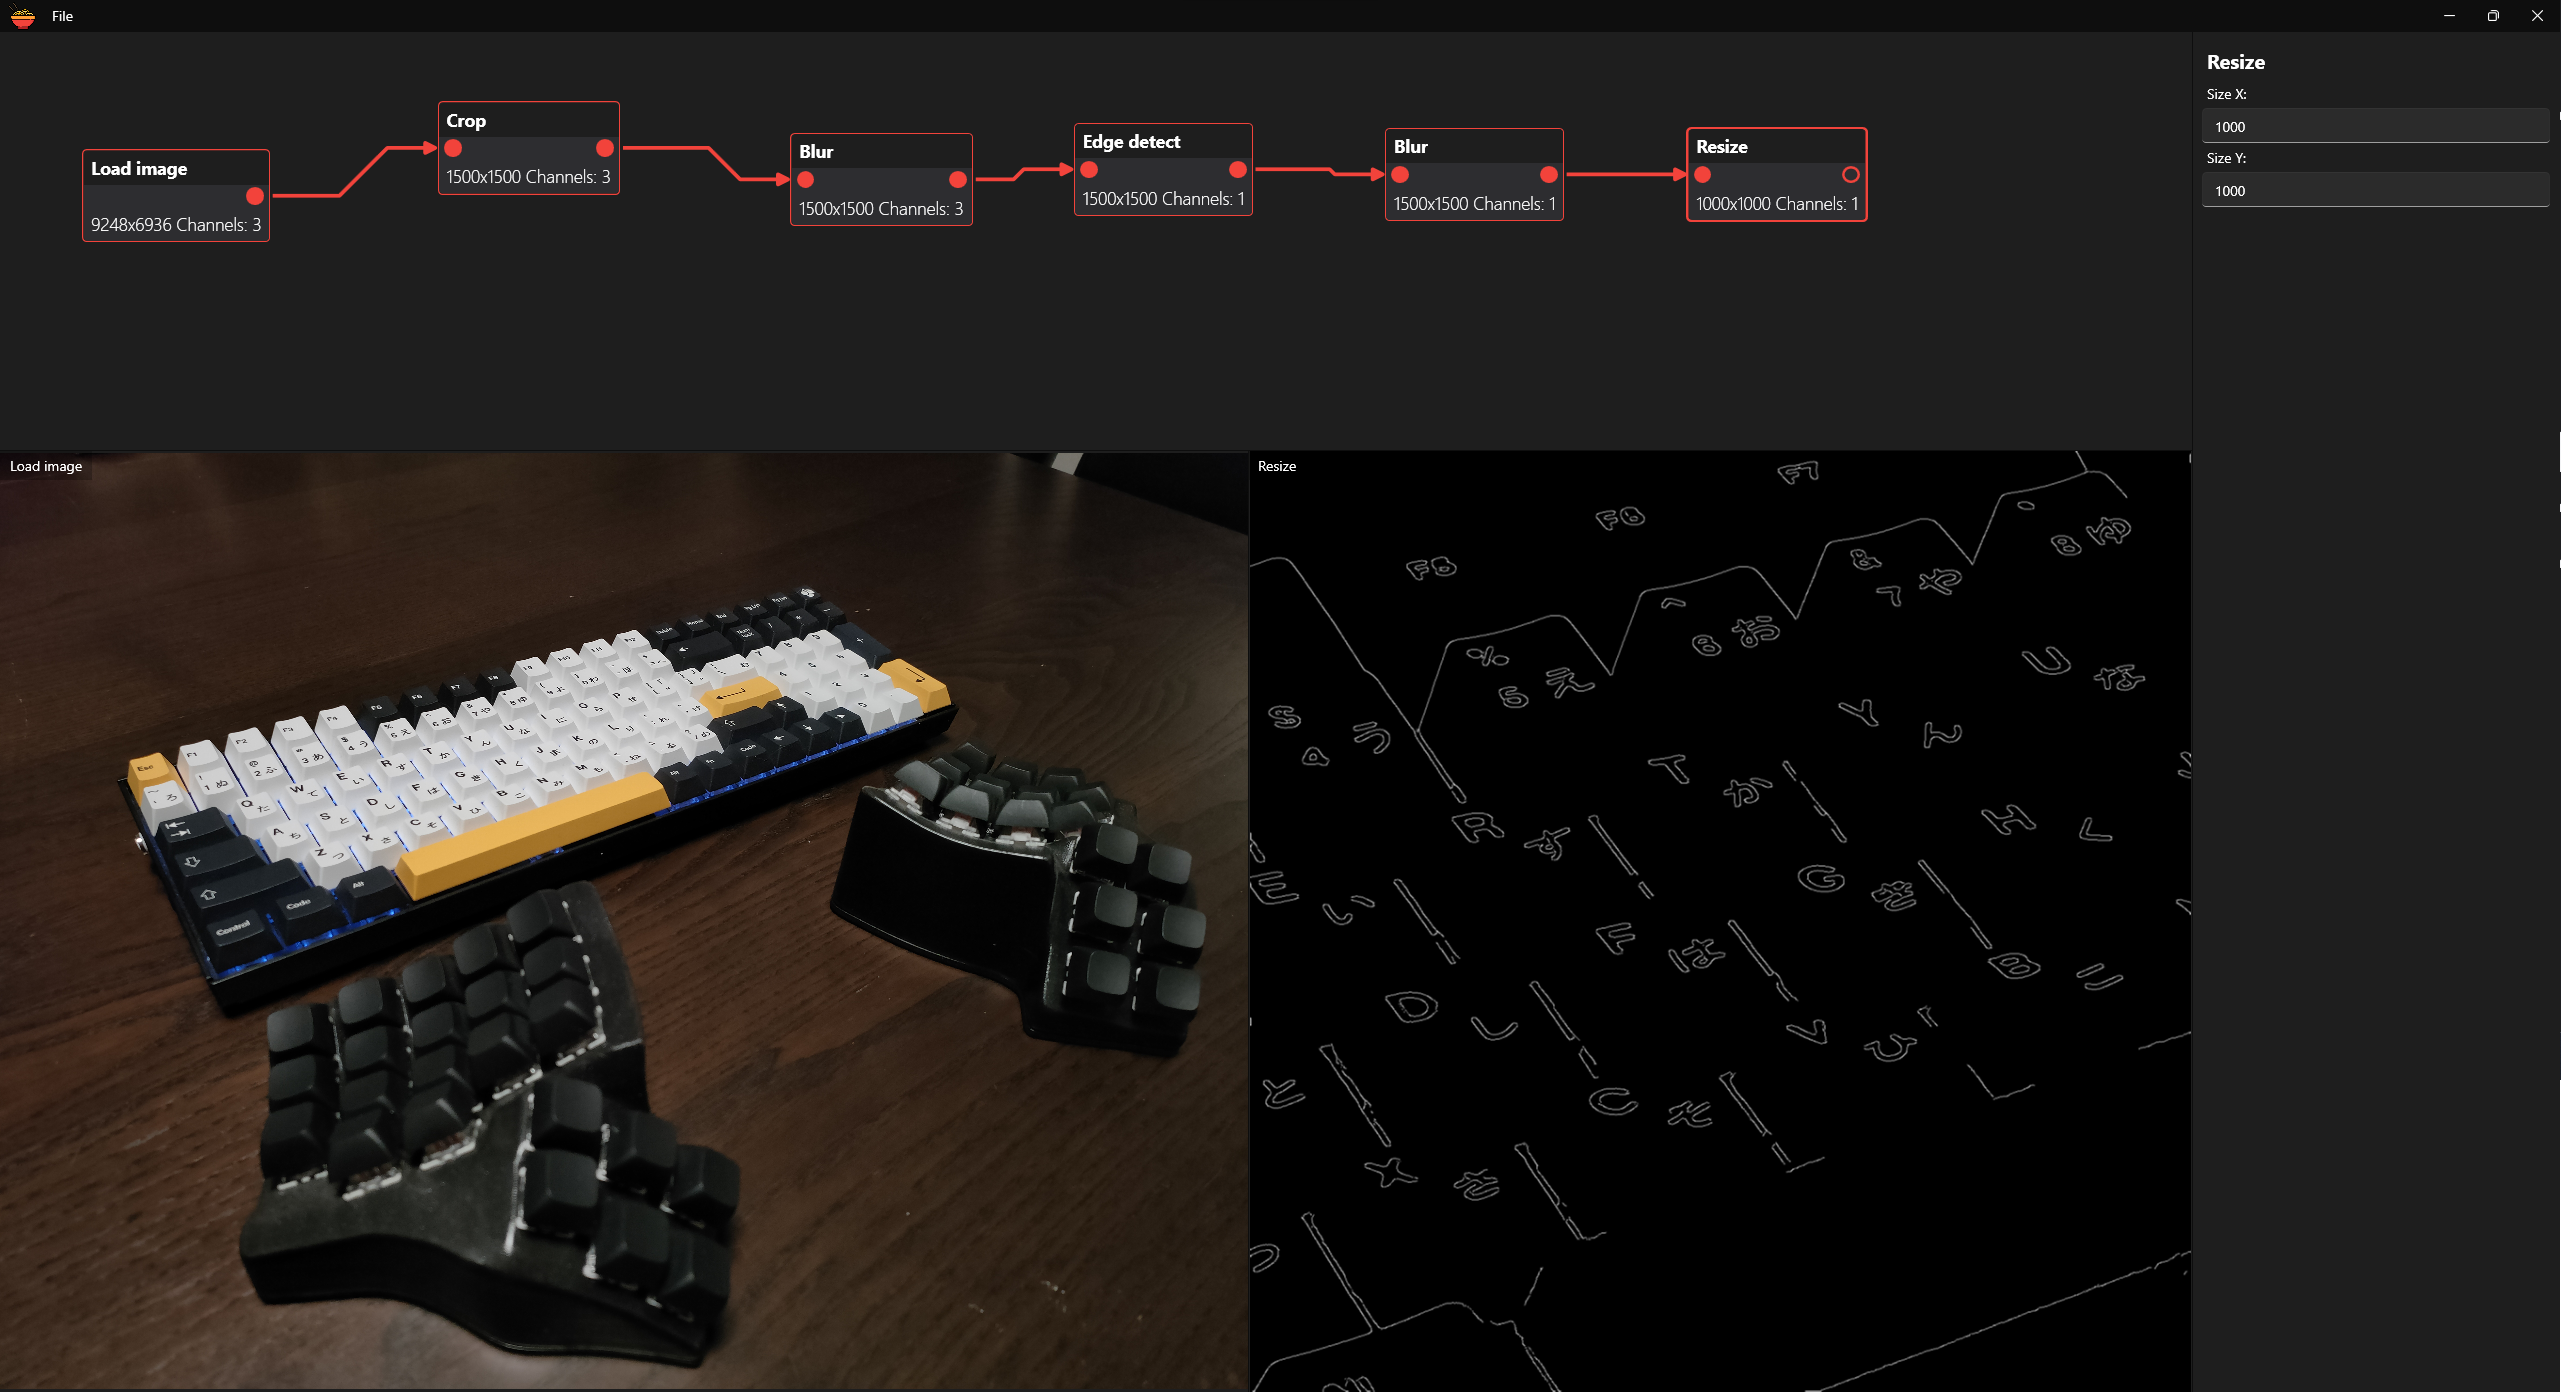
\includegraphics[width=1\linewidth]{images/Picture28.png}
    \caption{Wykrywanie krawędzi dla uwydatnienia liter. Opracowanie własne.}
    \label{fig:keyboard}
\end{figure} 

\begin{figure}[H]
    \centering
    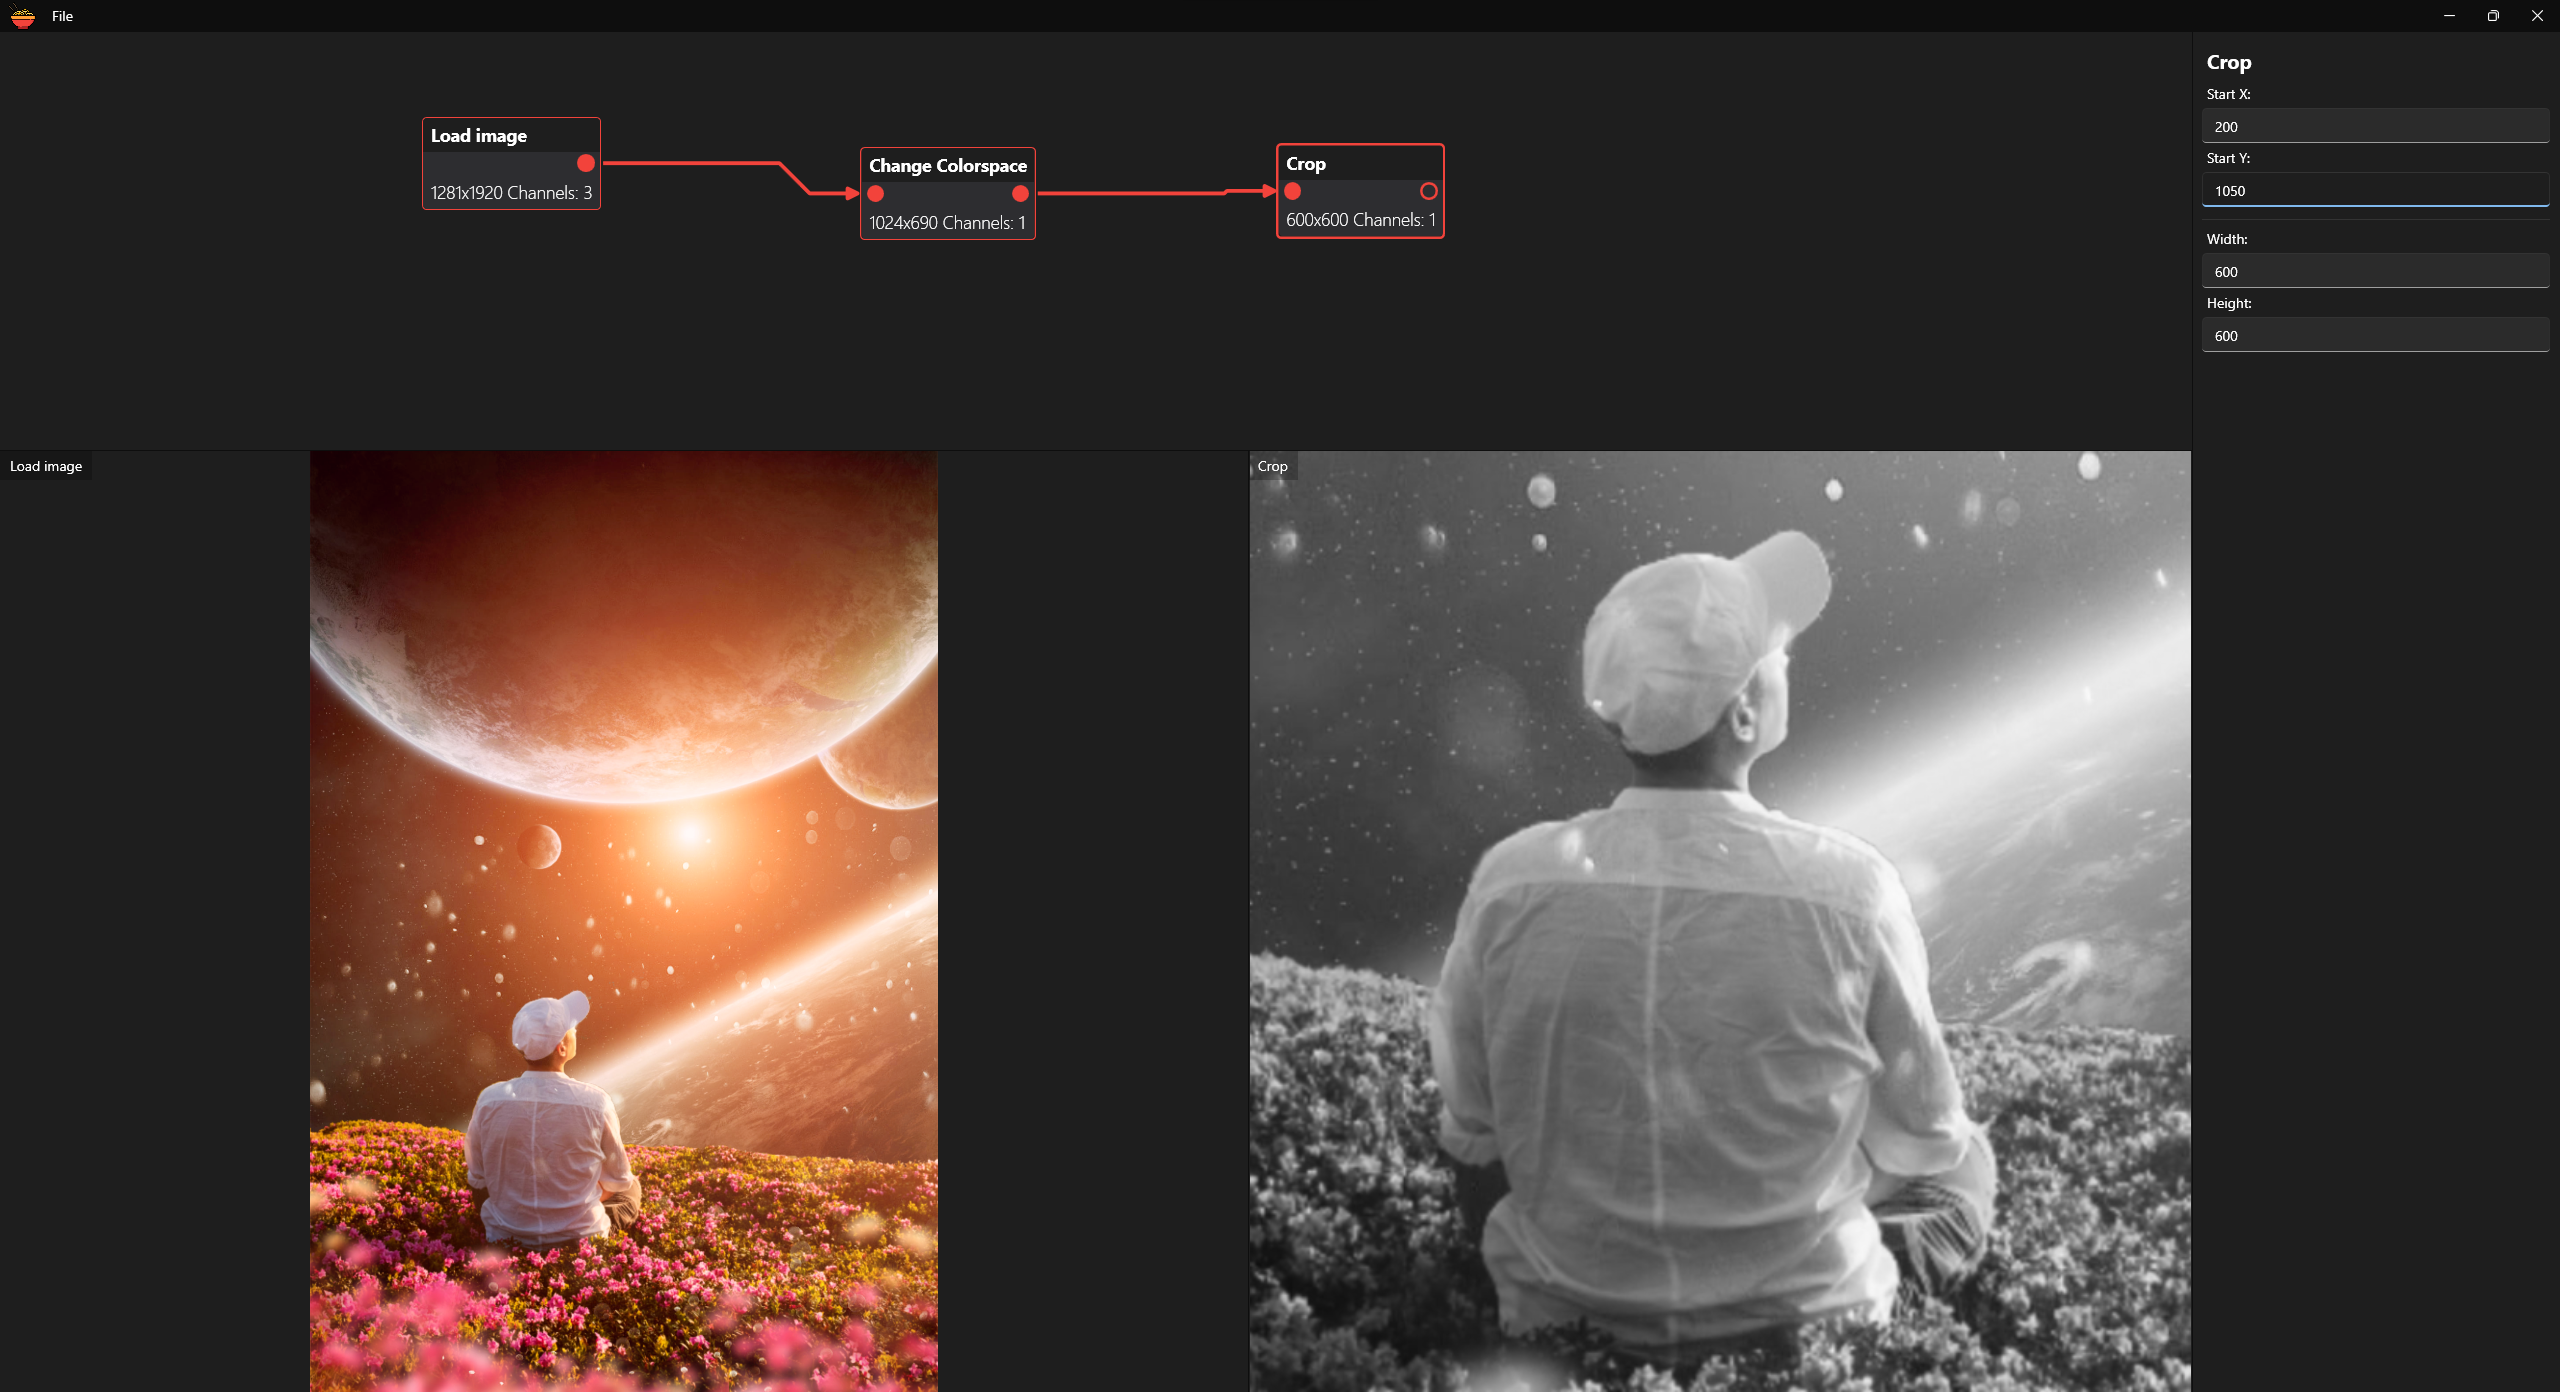
\includegraphics[width=1\linewidth]{images/Picture29.png}
    \caption{Obcięcie zdjęcia i zmiana na odcienie szarości. Opracowanie własne.}
    \label{fig:person}
\end{figure} 

\begin{figure}[H]
    \centering
    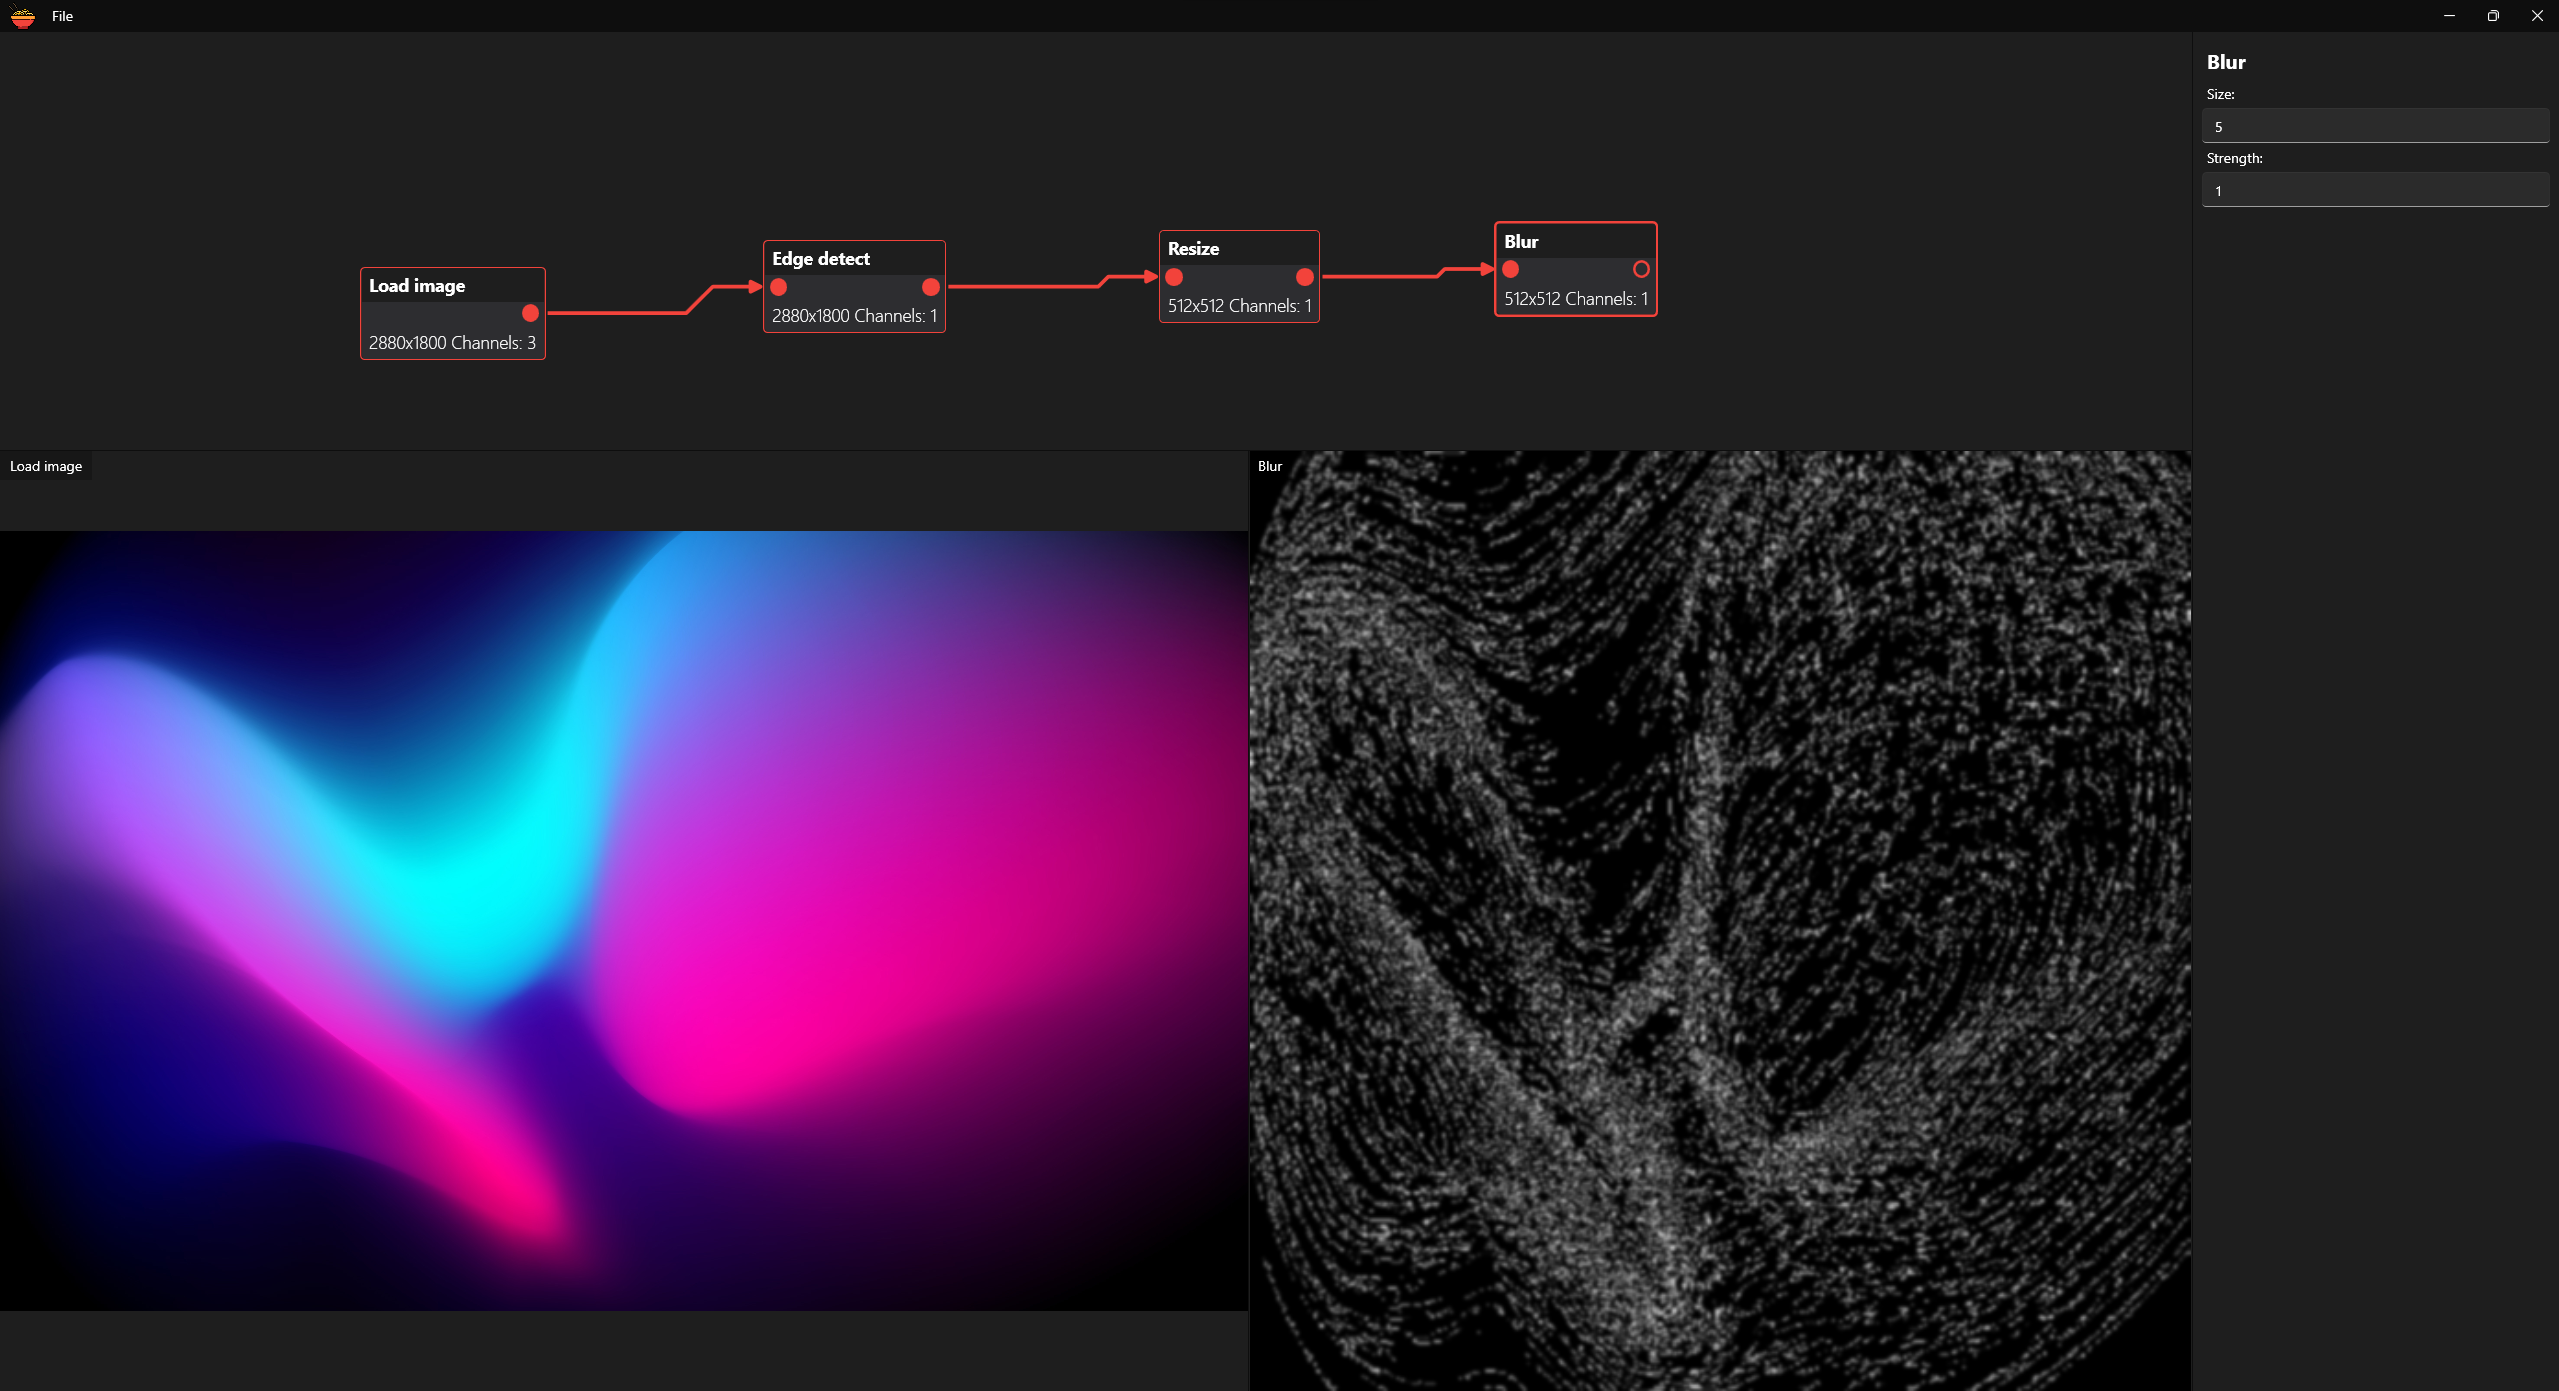
\includegraphics[width=1\linewidth]{images/Picture30.png}
    \caption{Abstrakcyjne edytowanie. Opracowanie własne.}
    \label{fig:abstract}
\end{figure} 